\documentclass[french]{beamer}
\usepackage{comment}
\usepackage[utf8]{inputenc}
\usepackage[T1]{fontenc}
\usepackage{lmodern}
\usepackage{amsmath, amssymb}
\usepackage{multimedia}
\usepackage{babel}
\usepackage{pgfplots}
\usetheme[width=2cm]{PaloAlto}
\usepackage{graphicx}
\usepackage{subcaption}
\usepackage{textpos}
\usepackage{mathrsfs}
\usetikzlibrary{patterns}
\pgfplotsset{compat=1.15}
\usetikzlibrary{arrows}
\usepackage{multimedia}
\usepackage{pdfpages}
\usepackage{algorithm}
\usepackage{algorithmic}
\title{A Regularized Wasserstein Framework for Graph Kernels }
\subtitle{Asiri Wijesinghe, Qing Wang, and Stephen Gould
School of Computing, Australian National University, Canberra, Australia}
\author{Grégoire Béchade}
\date{January 16 2025}




\begin{document}


% title :
\begin{frame}
\titlepage
\end{frame}


\section{Introduction}
\begin{frame}{Introduction}

    \begin{enumerate}
        \item A measure to compare graph similarity
        \item Numerical experiments
    \end{enumerate}

\end{frame}

\section{A measure to compare graph similarity}

\begin{frame}{From graphs to distributions}
    In order to compare graphs with Wasserstein distance, we need to associate each graph with a distribution.
    Let : \\
    \begin{itemize}
        \item  $\xi_f : V \rightarrow \mathbb{R}^m$ a feature embedding of the nodes\\
        \item $\xi_s : V \rightarrow \mathbb{R}^k$ a structure embeding of the nodes
    \end{itemize}

$p = \sum_{i=0}^{n} \mu_i \delta(\xi_f(v_i), \xi_s(v_i))$ can be seen as a distribution on $\mathbb{R}^{m+k}$. 
    
\end{frame}

\begin{frame}{Defining the Wasserstein problem}

    To solve a Wasserstein problem, one need to define a cost function : \\[0.3cm]

    $C^V(i,j) = \lVert (\xi_f(v_i), \xi_f(v_j)) \rVert ^2   $\\[0.3cm]

    With $ \xi_f (v_i)$ the feature embedding of the node $v_i$:\\[0.3cm]
    $\xi_f(v_i) = [x_i, \Delta(x_i)] \in \mathbb{R}^{2m}$ and $ \Delta(x_i)$ the local variation of the node $x_i$. \\[0.3cm]
    
\end{frame}



\begin{frame}{LW: A Regularization to Preserve Neighborhood Similarity}
        \textbf{LW distance:}
        \[
        LW(\mu, \nu) = \underset{\gamma}{\operatorname{min}} \left\langle \gamma , C^N \right\rangle_F + \Theta_\omega(\gamma) 
        \]\\
$ C^N(i,j) = d_s(e_i, e_j)$, with $e_i$ and $e_j$ the embeddings of the nodes $v_i$ and $v_j$\\[0.3cm]
$ \Theta_w(\gamma) = \lambda_\mu \Gamma_\mu(\gamma) + \lambda_\nu \Omega_\nu(\gamma) = \frac{\rho}{2}{ \lVert \gamma\rVert _F}^2$
\end{frame}

\begin{frame}{LW: A Regularization to Preserve Neighborhood Similarity}

    $\hat{e_i}$ : mean of the embeddings of the nodes connected to $v_i$ in $\gamma$ : \\[0.3cm]
$ \hat{e}_i^\mu = \frac{\sum_{j=1}^{n_2} \gamma(i,j)e_j^{\nu}}{\sum_{j=1}^{n_2} \gamma(i,j)}$. \\[0.3cm]

\textbf{Source regularization} : $\Omega_\mu(\gamma) = \frac{1}{n_1^2} \sum_{i,j} a_{i,j} \left\lVert \hat{e}_i^\mu - \hat{e}_j^\mu\right\rVert ^2 $, with $a_{i,j}$ the adjacency matrix of $G_1$.\\[0.3cm]
\textbf{Target regularization} : Defined the same way. 


\end{frame}
\begin{frame}{GW: A Regularization to Preserve Pairwise Similarity}
    \begin{itemize}
        \item \textbf{Pairwise similarity:}
        \begin{itemize}
            \item Cost matrix for graph \( G \): \( C^P(i,j) = d_s(e_i, e_j) \).
            \item Pairwise similarity between \( G_1 \) and \( G_2 \):  
            \[
            L_2(C_1^P(i,j), C_2^P(k,l)) = \left\lvert C_1^P(i,j) - C_2^P(k,l) \right\rvert^2
            \]
        \end{itemize}

        \item \textbf{Gromov-Wasserstein (GW) distance:}
        \[
        GW(\mu, \nu) = \underset{\gamma \in \pi(\mu, \nu)}{\operatorname{min}} \left\langle \gamma, L_2(C_1^P, C_2^P) \otimes \gamma \right\rangle_F - \lambda_g \Theta_g(\gamma)
        \]
        \begin{itemize}
            \item \(\Theta_g(\gamma)\): Kullback-Leibler divergence with prior \( \gamma' \).
            \item Regularization improves convergence despite GW not being convex.
        \end{itemize}

    \end{itemize}
\end{frame}

\begin{frame}{solving this optimization problem with the SCG algorithm}
    \begin{itemize}
        \item NP-hard problem. 
        \item SCG algorithm that iterates by using the gradient of the objective function as the cost matrix in a Sinkhorn-Kopp algorithm.
        \item Theoretical guarantees of the convergence. 
    \end{itemize}
    
\end{frame}

\begin{frame}{Using This distance to perform graph classification}

    The authors use kernel methods to classify graphs:\\[0.3cm]
    $K(G_1, G_2) = e^{(-\eta RW(G_1, G_2))}$\\[0.3cm]

    Which is not positive definite but is seen as the noisy observation of a positive definite kernel.\\[0.3cm]
\end{frame}

\begin{frame}{Data used for numerical experiments}

\begin{itemize}
    \item Task : classification of 2-nn and 3-nn graphs.\\[0.3cm]
    \item Train set : 400 graphs
    \item Test set : 100 graphs
    \item Balanced classes 
\end{itemize}

\begin{figure}[h]
    \centering
    \begin{subfigure}{0.4\textwidth}
        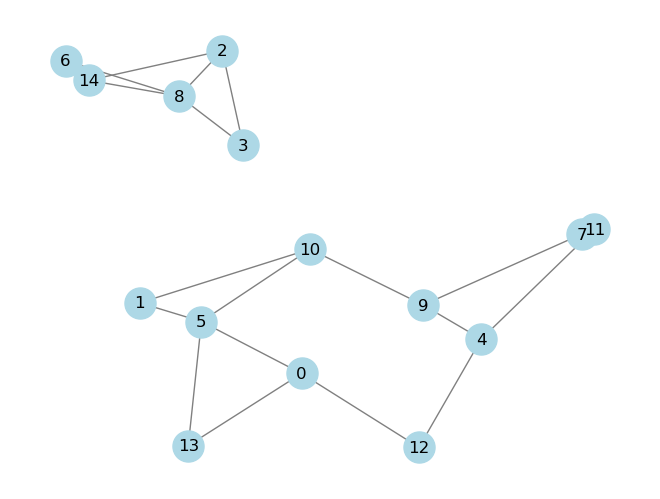
\includegraphics[width=\textwidth]{figures/graph_k2.png}
        \caption{Example of a graph with k = 2 }
    \end{subfigure}
    \begin{subfigure}{0.4\textwidth}
        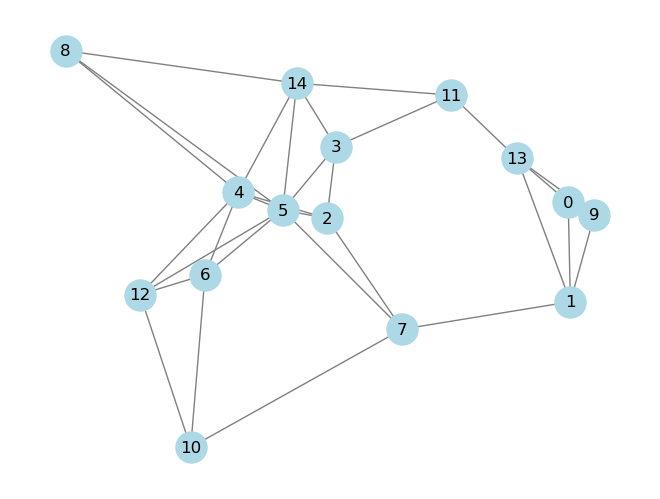
\includegraphics[width=\textwidth]{figures/graph_k3.png}
        \caption{Example of a graph with k = 3}
    \end{subfigure}
    \caption{Example of two graphs of each class}
\end{figure} 

\end{frame}

\begin{frame}{Impact of the different parameters }

I have studied the impact of the different parameters on this simple task. 
    
\begin{table}[h]
    \centering
    \begin{tabular}{|c|c|c|c|c|}
        \hline
        & Time (min) & F1-score & Accuracy \\
        \hline
        Default & 47 & 0.65 & 0.73 \\
        \hline
        $\beta_2/\lambda_g = 0$ & 25 & 0.78 & 0.76 \\
        \hline
        $\rho = 0$ & 62 & 0.63 & 0.71 \\
        \hline
        $\lambda_\mu = 0$ & 58 & 0.65 & 0.71 \\
        \hline
        $\lambda_\nu = 0 $ & 32 & 0.65 & 0.72 \\
        \hline
        $\lambda_g = 0$ & 38 & 0.61 & 0.69 \\
        \hline
        Sinkhorn algorithm  & 11 & 0 & 0.5 \\
        \hline
        Random Forest &$ 2.10^{-2}$& 0.63 & 0.67\\
        \hline
        SVC Gaussian kernel  &0 &0.60 & 0.66 \\
        \hline
        KNN & 1 & 0.7 & 0.68 \\
        \hline
    \end{tabular}
    \caption{Performances of the classifier with different variations}
    \label{tab:results}
\end{table}
    
\end{frame}

\begin{frame}{Impact of the two regularization terms}

    \begin{figure}[h]
        \centering
        \begin{subfigure}{0.32\textwidth}
            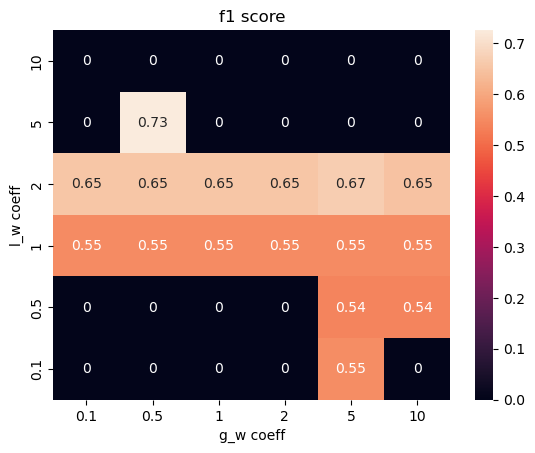
\includegraphics[width=\textwidth]{figures/f1_score_results.png}
            \caption{F1-score}
            \label{fig:f1_score}
        \end{subfigure}
        \begin{subfigure}{0.32\textwidth}
            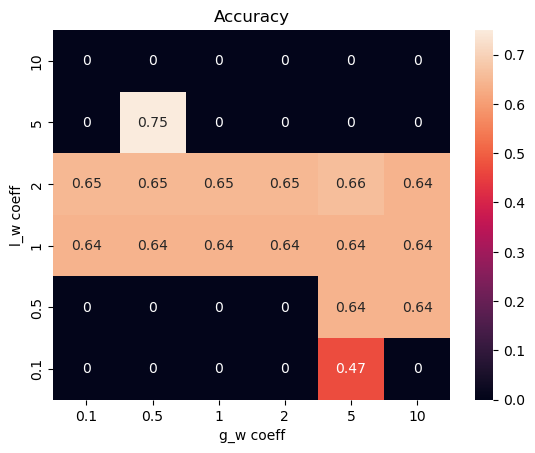
\includegraphics[width=\textwidth]{figures/accuracy_results.png}
            \caption{Accuracy}
            \label{fig:accuracy}
        \end{subfigure}
        \begin{subfigure}{0.32\textwidth}
            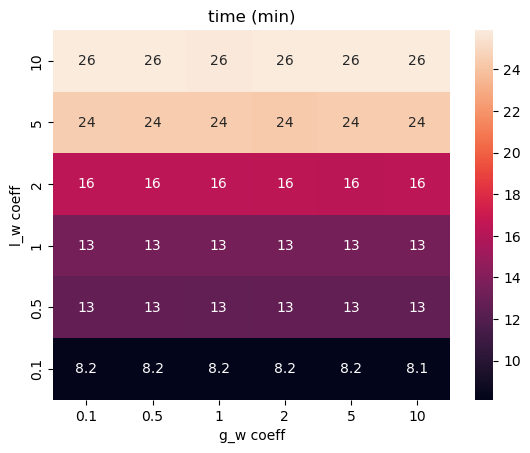
\includegraphics[width=\textwidth]{figures/time_results.png}
            \caption{Computational time}
            \label{fig:time}
        \end{subfigure}
        \caption{Results of the classifier with variations of the two regularization terms}
    \end{figure}
    
\end{frame}
\section{Conclusion}
\begin{frame}{Conclusion}
\begin{itemize}
    \item An complete way to determine the similarity between graphs. 
    \item Results of the paper not reproduced on a single classification task. 
\end{itemize}
\end{frame}

\end{document}
